\pagestyle{empty}


\begin{tikzpicture}[remember picture, overlay]
    \node[
        shape = rectangle,
        minimum height = \paperheight,
        minimum width = \paperwidth,
        anchor = south west,
        fill = blue!5]
        (sheet) at (current page.south west) {};
    \tikzset{shift = {(sheet.center)}}
    \node at (0, -2) {
        \HUGE
        \begin{tabular}{c}
            \textsc{Теория информации}\\
            \huge Конспект лекций
        \end{tabular}
    };

    \node[inner sep = 0pt, opacity = 0.5] at (6, 10.5){
        
\includegraphics[width = 0.27\textwidth] {pics/sun.png}
    };


    \begin{scope}[shift = {(0, 3)}]
        \node[inner sep = 0pt, opacity = 0.5] at (-5, 0){
            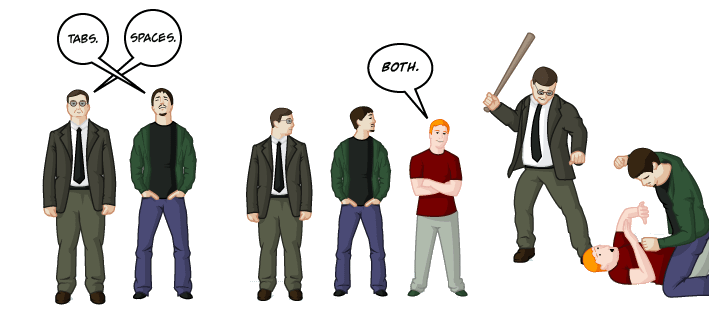
\includegraphics[width = 0.4\textwidth] {pics/tabs-spaces.png}
        };
        \node[inner sep = 0pt, opacity = 0.5] at (-5, -2.3){
            \textsc{Коммуникационная сложность}
        };
        \node[inner sep = 0pt, opacity = 0.5] at (5, 0){
            
\includegraphics[width = 0.4\textwidth] {pics/bender.png}
        };
        \node[inner sep = 0pt, opacity = 0.5] at (5, -2.3){
            \textsc{Колмогоровская сложность}
        };
    \end{scope}

    \begin{scope}[shift = {(0, -8)}]
        \node[inner sep = 0pt, opacity = 0.5] at (0, 0){
            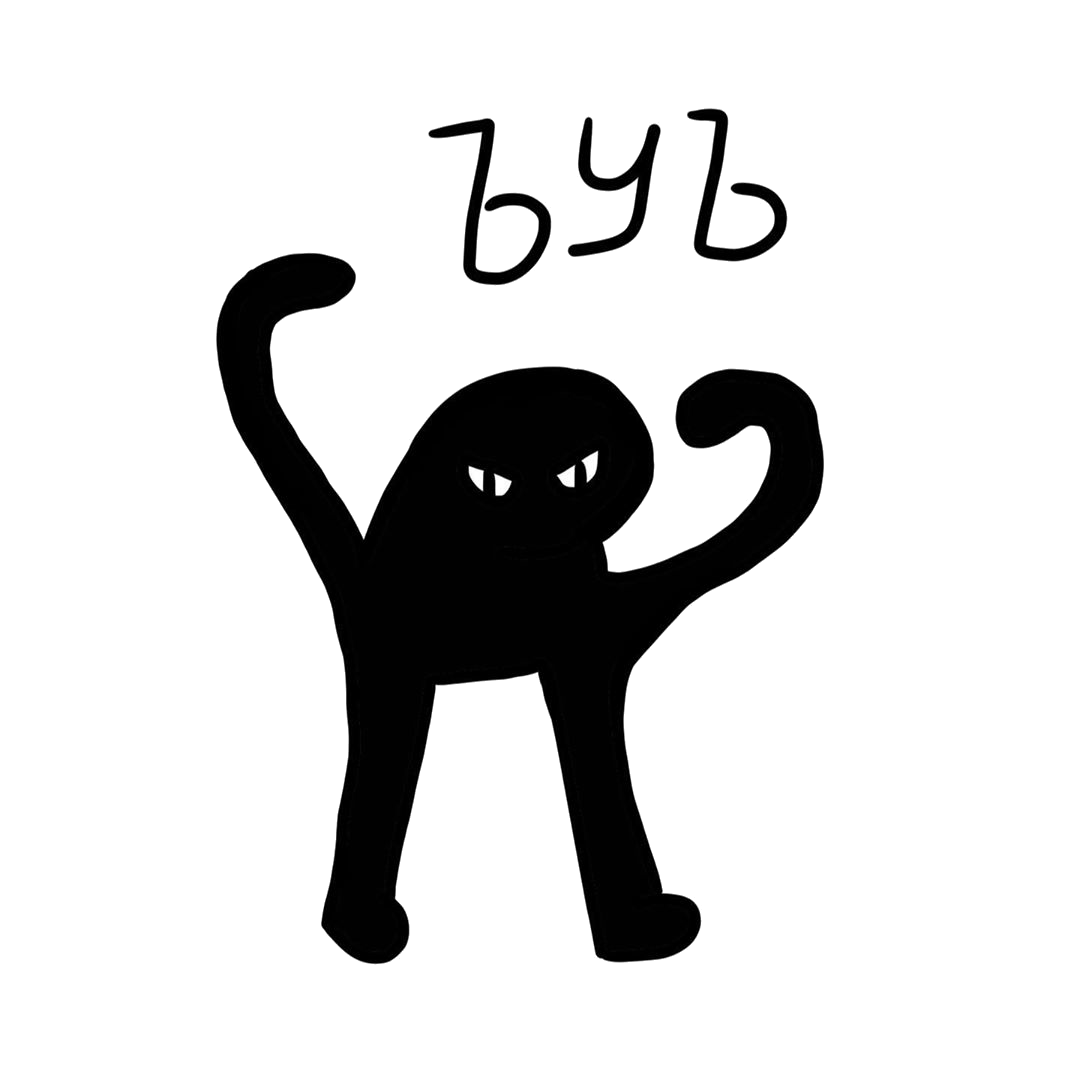
\includegraphics[width = 0.5\textwidth] {pics/uuu.png}
        };
        \node[inner sep = 0pt, opacity = 0.5] at (0, -4.2){
            \textsc{Теория кодирования}
        };
    \end{scope}


%    \pic[scale = 1.6] at (-3.5, -5) {tikzart-gun};

%    \pic[scale = 1.6] at (7, -9) {tikzart-bunny};
%    \pic[scale = 1.6] at (-5, 5) {tikzart-bunny};
%    \pic[scale = 1.6, rotate = 40] at (-5, -8) {tikzart-bunny};
%    \pic[scale = 1.6, rotate = -10, xscale = -1] at (6, 1) {tikzart-bunny};
%    \pic[scale = 1.6, rotate = 30, xscale = -1] at (8, 9) {tikzart-bunny};

%    \draw[platform] (\paperwidth / 2, -12.02) -- ++(-\paperwidth, 0);

%    \foreach \i in {0, 1, ..., 4}{
%        \pic[scale = 4] at (-5 + 1.8 * \i, -12) {tikzart-train};
%        \draw (-3.2 + 1.8 * \i, -11.7) -- ++(-0.2, 0);
%    }
%    \pic[scale = 4] at (-5 + 1.8 * 5, -12) {tikzart-trainhead};
\end{tikzpicture}


\clearpage
